\documentclass[12pt]{article}
\usepackage{graphicx}
%\documentclass[journal,12pt,twocolumn]{IEEEtran}
\def\inputGnumericTable{}
\usepackage{color}                                            %%
    \usepackage{array}                                            %%
    \usepackage{longtable}                                        %%
    \usepackage{calc}                                             %%
    \usepackage{multirow}                                         %%
    \usepackage{hhline}                                           %%
    \usepackage{ifthen}
\usepackage[none]{hyphenat}
\usepackage{graphicx}
\usepackage{listings}
\usepackage[english]{babel}
\usepackage{graphicx}
\usepackage{caption} 
\usepackage{hyperref}
\usepackage{booktabs}
\usepackage{array}
\usepackage{amsmath}   % for having text in math mode
\usepackage{listings}
\lstset{
  frame=single,
  breaklines=true
}
  
%Following 2 lines were added to remove the blank page at the beginning
\usepackage{atbegshi}% http://ctan.org/pkg/atbegshi
\AtBeginDocument{\AtBeginShipoutNext{\AtBeginShipoutDiscard}}
%


%New macro definitions
\newcommand{\mydet}[1]{\ensuremath{\begin{vmatrix}#1\end{vmatrix}}}
\providecommand{\brak}[1]{\ensuremath{\left(#1\right)}}
\providecommand{\norm}[1]{\left\lVert#1\right\rVert}
\newcommand{\solution}{\noindent \textbf{Solution: }}
\newcommand{\myvec}[1]{\ensuremath{\begin{pmatrix}#1\end{pmatrix}}}
\let\vec\mathbf

\begin{document}

\begin{center}
\title{\textbf{Properties of Collinear}}
\date{\vspace{-5ex}} %Not to print date automatically
\maketitle
\end{center}

\setcounter{page}{1}

\section{10$^{th}$ Maths - Chapter 7}

This is Problem-2 from Exercise 7.3.2

\begin{enumerate}
\item In each of the following find the value of ‘k’, for which the points are collinear.
\end{enumerate}
\begin{enumerate}
\item (7, –2), (5, 1), (3, k) \\
\item (8, 1), (k, – 4), (2, –5).\\
\end{enumerate}
\section{Solution for problem :1}
\begin{align}
\vec{D} &=\brak{\vec{A}-\vec{B}} = \brak{\myvec{7 \\-2 } - \myvec{5 \\1 } } = \myvec{2 \\ -3 }\\
\vec{E} &= \brak{\vec{A}-\vec{C}} = \brak{\myvec{7 \\ -2 } - \myvec{3 \\K } } = \myvec{4 \\1\-2-K}
\end{align}

If  points on a line  are  collinear, rank of matrix is " 1 "then the vectors are in linearlydependent.
For 2 × 2 matrix Rank =1 means Determinant is 0.

Through pivoting,we obtain
\begin{align}
\vec{F} &={\myvec{\vec{D}\\ \vec{E}}}\\
\begin{pmatrix}
2 & -3 \\
4 & -2-k 
\end{pmatrix}
\end{align}
\begin{align}
\begin{pmatrix}
2 & -3 \\ 
 4& -2-k
\end{pmatrix}\overset{R2=R2-2R1}{\rightarrow}
\begin{pmatrix}
-2-k &-4 \\ 
 4& -2-k
\end{pmatrix}
\end{align}

if the rank of the matrix is 1 means any one of the row must be zero.So, making the first element in the matrix to 0.

\begin{equation}
-2-k-2(-3)=0
\end{equation} 
\begin{equation}
-2-k-6=0\\
\end{equation} 
\begin{equation}
k=4 \\
\end{equation} 
Hence proved.
\begin{figure}[h!]
	  \centering 
	  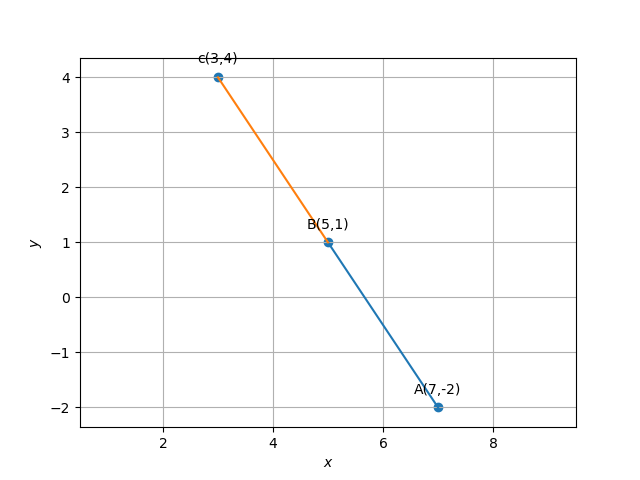
\includegraphics[width=\columnwidth]{line1.png}
	  \caption{}
	  \label{fig:line1.png}
	  \end{figure} 	    
\section{Solution for problem :2}
\begin{align}  
\vec{A}=\myvec{8 \\ 1}
\vec{B}=\myvec{k \\ -4}
\vec{C}=\myvec{2 \\ -5}
\end{align}
\begin{align}  
 \vec{D} &=\brak{\vec{A}-\vec{B}} = \brak{\myvec{8 \\1 } - \myvec{k \\-4 } } = \myvec{8-k \\ 5 }\\
\vec{E} &= \brak{\vec{A}-\vec{C}} = \brak{\myvec{8 \\ 1 } - \myvec{2 \\-5 } } = \myvec{6 \\6}
\end{align}

If points on a line  are  collinear, rank of matrix is " 1 "then the vectors are in linearlydependent.
For 2 × 2 matrix Rank =1 means Determinant is 0.

Through pivoting,we obtain

\begin{align}
\vec{F} &={\myvec{\vec{D}\\ \vec{E}}}\\
\begin{pmatrix}
8-k & 5 \\
6 & 6 
\end{pmatrix}
\end{align}
\begin{align}
\begin{pmatrix}
8-k & 5 \\ 
6& 6
\end{pmatrix}\overset{R1=3R1-R2}{\rightarrow}
\begin{pmatrix}
24-3k & 15 \\ 
 6& 6
\end{pmatrix}
\end{align}

if the rank of the matrix is 1 means any one of the row must be zero.So, making the first element in the matrix to 0.

\begin{equation}
3(8-k)-3(5)=0
\end{equation} 
\begin{equation}
24-3k-15=0\\
\end{equation} 
\begin{equation}
k=3 \\
\end{equation} 
Hence proved.
\begin{figure}[h!]
	  \centering 
	  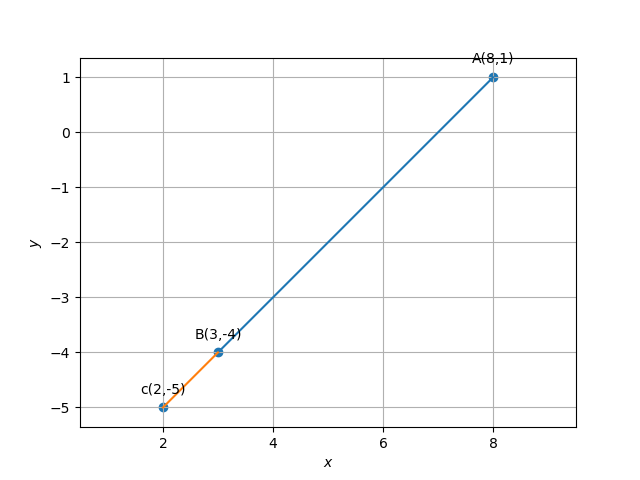
\includegraphics[width=\columnwidth]{line2.png}
	  \caption{}
	  \label{fig:line2.png}
	  \end{figure} 
\end{document}
